\section*{Preliminary}
\subsection{Implicit 3D reconstruction}
Implicit 3D reconstruction can be defined as follows. 
A sequence of captured views $\bm{v_n}=\{v_0, v_1, ..., v_n\} \subseteq \bm{v}$, where $v_i=\{I_i,p_i\}$, $I_i$ represents the image captured and $p_i$ represents the corresponding camera pose.
By assuming that training samples $v_i \in \bm{v_n}$ are independent of each other, we then optimize the whole latent codes $\theta=\{\theta_0,...,\theta_m\}$ by minimizing a loss function $L(\theta, \bm{v_n}) = \frac{1}{n}\sum_{i=0}^{n} f(\theta, v_i)$.
$f(\theta, v_i)$ is typically the negative log-likelihood between model output $r(\theta, p_i)$ and $I_i$, approximated by mean square error.
Grided implicit 3D reconstruction follows similar definitions except that multiple light weight$\theta$ are grouped together as a grid and each maps a small region of the 3D scene.
The grid of local latent codes are jointly optimized by summing up their loss functions.

\subsubsection{Next Best View}
When exploring a previously unknown environment, NBV for implicit 3D reconstruction aims to to find a view $v_{n+1}\in\bm{v}$ that maximize information gain:
\begin{equation}
    v_{n+1} = \mathop{\arg\max}\limits_{v,p\in v} g(\theta^n, p, \bm{v_n})
    \label{nbv2}
\end{equation}
where $\theta^n$ is the latent codes after optimization over $\bm{v_n}$ and the actual image $I\in v$ is unknown at this step.
There might be various possible definitions for $g(\cdot)$ that calculates information gain of a candidate view $v$, but they should fundamental be in proportion to the possible improvement to $\theta$ towards an optimal $\theta'$ that minimizes $L(\theta, \bm{v})$, which is intuitively the knowledge about the whole scene extracted from $v$:
\begin{equation}
    g(\theta^n, v, \bm{v_n}) \propto \sum_{i=0}^{m}(\lvert\theta'_i - \theta_i^n\rvert - \lvert \theta'_i - \theta_i^{\bm{v_n} + v}\rvert)
    \label{gain}
\end{equation}

\section{Methodology~\ref{methodology}}
% \subsection{Training-Time Uncertainty Estimation}
\subsection{Training-Time Uncertainty Estimation}
% Although grided implicit 3D reconstruction brings an extra uncertainty due to limited capacity of local latent codes, it also provides two good properties: local latent codes have clear 3D correspondence and local latent codes mapping simple local geometries easily converge to reasonable $\theta$ given $\bm{v_n}$.
\begin{figure*}
    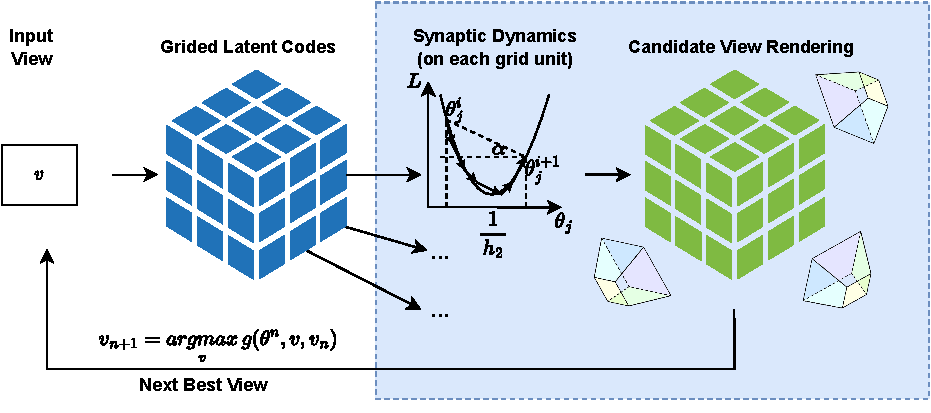
\includegraphics{overview.pdf}
    \caption{Overview of the training-time uncertainty estimation pipeline of SharpView. The left blue grid is the grid of local latent codes of grided implicit 3D reconstruction. The right green grid is the corresponding data grid to store the certainty estimation of each local latent codes and we directly estimate the information gain of each candidate view by directly rendering their certainty estimation in the camera frustum.}
    \label{overview}
\end{figure*}

To save the computation burden of model inference for estimating information gain for each view, we consider the information that can be directly extracted from the latent codes.
While it is difficult to compute $\theta_i^{\bm{v_n} + v}$ in equation (\ref*{gain}) since $I$ is unknown, inspired by parameter regularization methods~\cite{zenke2017continual} introduced in continual learning, we can find how certain (consolidated) $\theta_i^n$ is from the knowledge of $\bm{v_n}$ in previous training, which is intuitively inversely proportional to space for further changes of $\theta_i$.

Since the training set is iteratively appended during the NBV process, we view training on $\bm{v_i}$ as a task $T_i$ and consider the synaptic dynamics observed during this task.
Similar to~\cite{zenke2017continual}, we assume the training and optimization of $L(\cdot)$ and $\theta$ during a task as a continual process on time $t$, and an infinitesimal parameter update $\Delta\theta$ at time $t$ results in change in $L(\cdot)$ as 
\begin{equation}
    L(\theta + \Delta\theta, \bm{v_{i+1}}) - L(\theta, \bm{v_{i+1}}) \approx \sum_{j=0}^{m} \frac{\partial L}{\partial \theta_j} \Delta\theta_j 
\end{equation}
Assume $\theta^i$ and $\theta^{i+1}$  is computed at $t_i$ and $t_{i+1}$, there is 
\begin{equation}
\begin{split}
    L(\theta^{i+1}, \bm{v_{i+1}}) - L(\theta^i, \bm{v_{i+1}}) 
        & \approx\sum_{j=0}^{m}\int_{t_i}^{t_{i+1}} \frac{\partial L}{\partial \theta_j(t)} \Delta \theta_j(t) \d t \\
        & = \sum_{j=0}^{m} \omega_j^{i+1}
\end{split}
\label{path}
\end{equation}
The right part of equation (\ref{path}) is equivalent to the path integral of the gradient along the parameter trajectory from $\theta^{i}$ to $\theta^{i+1}$.
It associates the records of gradients and parameter updates of each parameter (synaptic dynamics) with change in loss function and represents parameter specific contribution to changes in the total loss.
In practice, we can approximate $\omega_j^{i+1}$ using gradients and model updates computed during iterative mini-batch training.

Since we are assuming efficient training on grided implicit 3D reconstruction, we assume $L(\theta^{i+1}, \bm{v_{i+1}}) - L(\theta^i, \bm{v_{i+1}})$ correctly extracts knowledge from $\bm{v_{i+1}}$, which means $\omega_j^{i+1}$ can be used as evidence about how much $\bm{v_{i+1}}$ consolidate $\theta_j^{i+1}$.
However, since $\omega_j^{i+1}$ is dependent to $\lvert\theta_j^{i+1} - \theta_j^{i}\rvert$, we cannot directly use it as a comparison metric across different parameters.
Instead, we model the certainty of $\theta_j^{i+1}$ from $\bm{v_i}$ as the multiplication of two dimensionless factors, influence factor $h_1$ and concentration factor $h_2$.

% \begin{figure}
%     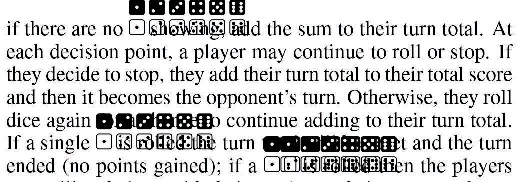
\includegraphics{figure1.pdf}
%     \caption{Synaptic Dynamics}
%     \label{dyn}
% \end{figure}

Let us consider the relationship between $L(\cdot)$ and $\theta_j$ by fixing other parameters in $L(\cdot)$ and we can get $L'(\theta_j, \bm{v_n})$.
% Assume the loss function can be approximated as $L(\theta, \bm{v_n})\approx \sum_{j=0}^{m} L'(\theta_j, \bm{v_n})$.
Since $\frac{L'(\theta_j^{i+1}, \bm{v_{n+1}}) - L'(\theta_j^i, \bm{v_{n+1}})}{\theta_j^{i+1} - \theta_j^{i}} \approx \tan \alpha$, where $\alpha$ represents the slope of $L'(\cdot)$ when $\theta_j$ varies from $\theta_j^i$ to $\theta_j^{i+1}$, we have 
\begin{equation}
h_1(\theta_j^{i+1}, \omega_j^{i+1}) = e^{\beta_j^{i+1}} - 1
\end{equation}
where$\beta_j^{i+1} = \frac{\omega_j^{i+1}}{\theta_j^{i+1}- \theta_j^{i}} \approx \frac{1}{\cos \alpha}$
because $\omega_j^{i+1}$ represents the path trajectory. This is depicted in the synaptic dynamics part in Fig.~\ref*{overview}. 
Intuitively, larger slope (smaller $\cos \alpha$) means $\theta_j$ is more influential to the loss function and a larger value for $h_1(\cdot)$, making us more certain about $\theta_j^{i+1}$ while a slope close to zero adds not confidence about $\theta_j^{i+1}$.

For the concentration factor, we have \begin{equation} 
    h_2(\theta_j^{i+1})=\frac{1}{\theta_j^{i+1} - \theta_j^{i}} = \frac{sign(\theta_j^{i+1} - \theta_j^{i})}{\lvert \theta_j^{i+1} - \theta_j^{i} \rvert}
\end{equation}
where $\frac{1}{\lvert \theta_j^{i+1} - \theta_j^{i} \rvert}$ estimates how concentrated $\theta_j$ is and higher level of concentration (smaller $\lvert \theta_j^{i+1} - \theta_j^{i} \rvert$) intuitively represents higher certainty.
$sign(\theta_j^{i+1} - \theta_j^{i})$ estimates sign of $\theta_j^{i+1} - \theta_j^{i}$ to maintain the information about the optimization direction, in case that the optimization direction disagrees between certain tasks. 
For example, in a task $T_i$, $\theta_j^{i+1} > \theta_j^{i}$ and in another task $T_j$, $\theta_j^{i+1} < \theta_j^{i}$ would cause us to be less confident about $\theta_j^{i+1}$.

Finally, we have the certainty estimation of $\theta_j^{i+1}$:
\begin{equation}
    c_j^{i+1}=(e^{\beta_j^{i+1}} - 1) \cdot \frac{sign(\theta_j^{i+1} - \theta_j^{i})}{\lvert \theta_j^{i+1} - \theta_j^{i} \rvert + \epsilon}
    \label{certain}
\end{equation}
which is mostly a multiplication of $h_1(\cdot)$ and $h_2(\cdot)$, and a dampening factor $\epsilon$ is added in case that $\theta_j^{i+1} - \theta_j^{i}$ is close to zero.
Summing up all the certainty estimation from training in the past, we have the certainty estimation of $\theta_j^{i+1}$ which is inversely proportional to information gain in equation (\ref*{gain})
\begin{equation}
    C(\theta_j^{i+1})=\lvert\sum_{k=0}^{i+1} c_j^k\rvert \propto \lvert\theta'_j - \theta_j^{i+1}\rvert - \lvert \theta'_j - \theta_j^{i}\rvert
    \label{Certain}
\end{equation}
Note that absolute value is used since different parameters can have different overall optimization direction.
In this way, we can maintain an online certainty (or rather, uncertainty) estimation of each parameter in $\theta$ by aggregating the synaptic dynamics during training and ease the burden of any extra training or inference.

\subsection{SharpView}
Leverage the certainty estimation of each parameter in equation~\ref{Certain}, we exploit the 3D correspondence relationship between local latent codes and the 3D scene that needs to be mapped to estimate information gain for NBV selection.
Intuitively, SharpView needs to find a view that visits local latent codes of the least certainty to maximize equation (\ref*{gain}).
However, for a view $v=\{I,p\}$, 3D correspondence of the local latent codes can be in three situations when rendered in $I$: empty without any geometries, having geometries rendered in $I$ and occluded without any geometries rendered in $I$.
Thus, we need to further carefully process $C(\theta_j^{n})$ to get an accurate estimation of information gain in a candidate view.
We define the set of local latent codes that are visible (not occluded) from any view in $\bm{v_n}$ as $\bm{\theta_{v_n}}$.
This can be easily computed by transforming the coordinates of the local latent codes to the camera frames, projecting them to $I$ using the intrinsic matrix of the camera and estimating whether their projections lie in $I$ and depth testing.

To distinguish the above three situations of (the 3D correspondence of) the local latent codes, we create a sparse data grid $G$ of the same 3D dimensions as the grid of local latent codes and assign three possible states (empty, surface and unknown) to the value of each data point on the grid.
$\theta_j \notin \bm{\theta_{v_n}}$ are marked as unknown by initializing the corresponding point on $G$ with a negative value.
A negative value is naturally smaller than any $C(\theta_j^{n})$ which is positive, and thus attract SharpView to explore unknown areas.
$\theta_j \in \bm{\theta_{v_n}}$ are first initialized with 0 and are updated by $C(\theta_j^{n})$ computed after training the latent codes over $\bm{\theta_{v_n}}$.
Typically, the training process of grided implicit 3D reconstruction only trains latent codes that lies around surfaces in the 3D scene to save computation.
As a result, $\theta_j$ lying in empty areas will be marked empty with a value of zero on $G$ and $\theta_j$ around surfaces will be marked surface with a positive $C(\theta_j^{n})$ value on $G$.

Given a candidate view $v=\{I,p\}$ where $I$ is unknown and data grid $G$ that stores the certainty estimation of the grid of local latent codes, we then render $G$ to $I'$ following the common rendering process of point cloud except treating unknown zones as surfaces $I'=Render(G,p)$, and average the non-zero values of $I'$ as the mean certainty estimation, ignoring the empty zones.
Summarizing the above process, our information gain estimation can be written as 
\begin{equation}
    g(\theta_n, v, \bm{v_n}) = -\frac{1}{K} \sum_{k=0}^{K-1} I''_k
    \label{ourgain}
\end{equation}
where $I'' = \{I'_k|I'_k\in I'\land  I'_k \neq 0\}$ and K is the size of $I''$.
With equation (\ref*{ourgain}), we can predict the information gain of $v$ via more light-weight and efficient point cloud rendering process compared with model inference, making SharpView suitable for edge devices that are limited in computation resources.
Equation (\ref*{ourgain}) guides the selection of NBV in equation (\ref*{nbv2}) to first cover the unknown areas and once unknown areas are mostly covered, revisit surfaces that are least certain, to get the greatest possible improvement of $\theta$.


% To distinguish the above three situations of (the 3D correspondence of) the local latent codes, we assign three possible states to the uncertainty estimation of a latent code
% we describe the process to store and update $C(\theta_j^{i+1})$ as follows.
% We assign three possible states 
% We first create a sparse data grid of the same 3D dimensions as the grid of local latent codes, which is meant to store the certainty estimation of each corresponding local latent codes.
% Second, to enable exploration in an unknown environment, we initialize the grid with a negative value to mark spots of unknown geometries not yet visited by $\bm{v_n}$.
% This value is naturally smaller than any $C(\theta_j^{i+1})$ which is positive, and thus attract SharpView to explore unknown areas.
% Then, to handle occlusion, given a sampled view $v$, we unproject $I$ back to the data grid to get surfaces.
% We mark the points whose 3D coordinates are after the rendered surfaces as occluded and mark the points before the rendered surfaces (empty) as empty.
% Finally, we update the data grid with the certainty estimation after training the latent codes over $\bm{v_n} + {v}$, and we ignore any update to those points marked as occluded in view $v$.
% We define the set of local latent codes that lie within the camera frustum from $p$ as $\bm{\theta_v}$ and the visible (not occluded) latent codes within the frustum as $\bm{\theta_v'} \subseteq \bm{\theta_v}$.
% $\bm{\theta_v}$ can be easily computed by transforming the coordinates of the local latent codes to the camera frame $p$, projecting them to $I$ using the intrinsic matrix of the camera and estimating whether their projections lie in $I$.






% \begin{equation}
% \begin{split}
%     v_{n+1} &= \mathop{\arg\max}\limits_{v,p\in v} g(\theta^n, p, \bm{v_n}) \\
%             &= \mathop{\arg\min}\limits_{v,p\in v} \sum_{\theta_j\in\bm{\theta_v}} C(\theta_j^{n})
% \end{split}
% \label{nbv3}
% \end{equation}



